\documentclass[10pt, xcolor=svgnames]{beamer}

\usepackage[T1]{fontenc}
\usepackage[utf8]{inputenc}
\usepackage{tikz}
\usepackage{verbatim}

\usetheme{Pittsburgh}
\usecolortheme{dove}

\title{Lattice Watering: Second Status Report}

\author{Christian Müller, Jonas Heinemann, Kaan Dönmez, Valentin Pickel}

\institute{
    Software Project on Internet Communication

    Summer Term 2022
    
    Freie Universität Berlin

    Institute for Computer Science
}

\date{June 13, 2022}

\begin{document}

\maketitle

\begin{frame}{Updates}
    \begin{itemize}
        \item The NIB did not seem to work last week, but we finally got around it on the 1st of June. So we were able to send CoAP packets from the BR to the host and, naturally, from the BR to nodes. What did not work was sending a packet to the host. The network setup is now automated and the routes are properly configured. Additionally, we setup RPL.
        \item We added the use of GCoAP.
        \item We added DTLS support.
        \item Added WDT to \texttt{br} and \texttt{fw}. (10 seconds max, 5 second refresh usually)
        \item We properly documented how the hardware is setup, especially how one can wire a node themselves.
        \item Added documentation on how to setup the hardware.
        \item We can remotely turn on the pump. This did work the last time, but it was rather messy to setup.
    \end{itemize}
\end{frame}

\begin{frame}[fragile]{RPL Topology}
    RPL (RFC 6550) states that for a home automation solution like ours, one root suffices:

    \begin{verbatim}
3.1.3.  Instances, DODAGs, and DODAG Versions

A RPL Instance contains one or more DODAG roots. A RPL Instance
may provide routes to certain destination prefixes, reachable
via the DODAG roots or alternate paths within the DODAG. ...

A RPL Instance may comprise:

o  a single DODAG with a single root

   *  For example, a DODAG optimized to minimize latency rooted at a
      single centralized lighting controller in a Home
      Automation application.
...
RIOT: gnrc_rpl_root_init(0, &ieee802154_ip, true, true);
    \end{verbatim}
\end{frame}

\begin{frame}[fragile]{Documented the HW Setup}
    \begin{verbatim}
HWSETUP.md
...
To build one of the node we used, you require:
        
1. One personal computer with the software set up.
2. Two SAMR21-XPRO boards, one bourder router and one node.
...
Connect the female jumpers the following way:

|   Device 1 | Connection 1 | Connection 2 |   Device 2 |
|------------|--------------|--------------|------------|
| SAMR21XPRO |          5V0 |          VCC |     DRV883 |
| SAMR21XPRO |          GND |          GND |     DRV883 |
| SAMR21XPRO |         PA13 |          IN1 |     DRV883 |
| SAMR21XPRO |         PA13 |          EEP |     DRV883 |
...
    \end{verbatim}
\end{frame}

\begin{frame}[fragile]{The Final Network Architecture}
    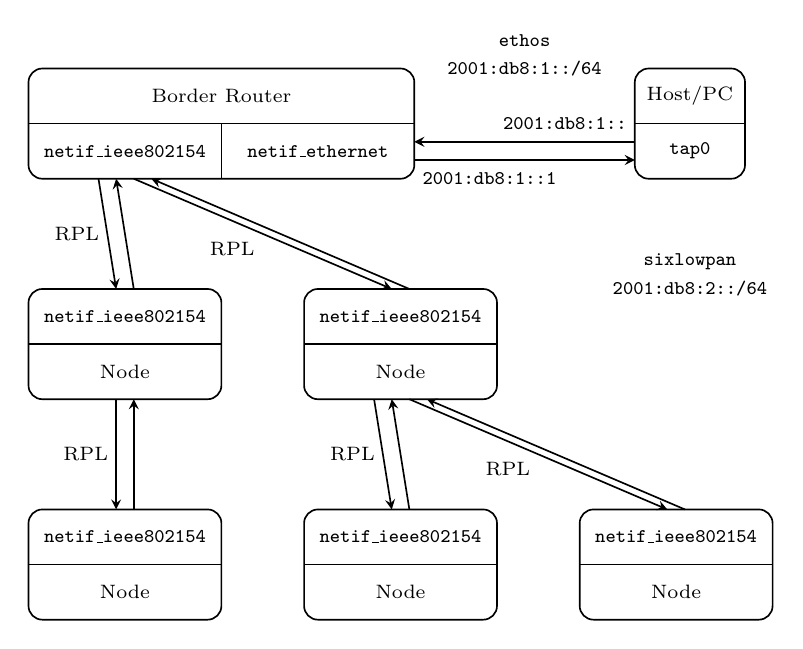
\begin{tikzpicture}[>=stealth, semithick, scale=0.7]
        \scriptsize
        \draw[rounded corners=5pt] (-1, -1) rectangle (1, 1);
        \draw[draw=none] (-1, 0) -- (1, 1) node[pos=0.5] {Host/PC};
        \draw (-1, 0) -- (1, 0);
        \draw[draw=none] (-1, 0) -- (1, -1) node[pos=0.5] {\texttt{tap0}};

        \draw[rounded corners=5pt] (-12, -1) rectangle (-5, 1);
        \draw[draw=none] (-12, 0) -- (-5, 1) node[pos=0.5] {Border Router};
        \draw (-12, 0) -- (-5, 0);
        \draw (-8.5, 0) -- (-8.5, -1);
        \draw[draw=none] (-12, 0) -- (-8.5, -1) node[pos=0.5] {\texttt{netif\_ieee802154}};
        \draw[draw=none] (-8.5, 0) -- (-5, -1) node[pos=0.5] {\texttt{netif\_ethernet}};
        \draw[->] (-1, -0.33) -- (-5, -0.33);
        \node[left] at (-1, 0) {\texttt{2001:db8:1::}};
        \node[right] at (-5, -1) {\texttt{2001:db8:1::1}};
        \node at (-3, 1.5) {\texttt{ethos}};
        \node at (-3, 1) {\texttt{2001:db8:1::/64}};
        \draw[->] (-5, -0.66) -- (-1, -0.66);

        \newcommand{\networknode}[2]{
            \draw[rounded corners=5pt] (#1, #2) rectangle (#1+3.5, #2-2);
            \draw (#1, #2-1) -- (#1+3.5, #2-1);
            \draw[draw=none] (#1, #2) -- (#1+3.5, #2-1) node[pos=0.5] {\texttt{netif\_ieee802154}};
            \draw[draw=none] (#1, #2-1) -- (#1+3.5, #2-2) node[pos=0.5] {Node};
        }

        \networknode{-12}{-3};
        \networknode{-7}{-3};
        \networknode{-12}{-7};
        \networknode{-7}{-7};
        \networknode{-2}{-7};

        \draw[->] (-12+1.75-0.48, -1) -- (-12+1.75-0.16, -3) node[left, pos=0.5] {RPL};
        \draw[->] (-12+1.75+0.16, -3) -- (-12+1.75-0.16, -1);
        \draw[->] (-12+1.75+0.16, -1) -- (-7+1.75-0.16, -3) node[below left, pos=0.5] {RPL};
        \draw[->] (-7+1.75+0.16, -3) -- (-12+1.75+0.48, -1);
        \draw[->] (-12+1.75-0.16, -5) -- (-12+1.75-0.16, -7) node[left, pos=0.5] {RPL};
        \draw[->] (-12+1.75+0.16, -7) -- (-12+1.75+0.16, -5);
        \draw[->] (-7+1.75-0.48, -5) -- (-7+1.75-0.16, -7) node[left, pos=0.5] {RPL};
        \draw[->] (-7+1.75+0.16, -7) -- (-7+1.75-0.16, -5);
        \draw[->] (-7+1.75+0.16, -5) -- (-2+1.75-0.16, -7) node[below left, pos=0.5] {RPL};
        \draw[->] (-2+1.75+0.16, -7) -- (-7+1.75+0.48, -5);

        \node at (0, -2.5) {\texttt{sixlowpan}};
        \node at (0, -3) {\texttt{2001:db8:2::/64}};
    \end{tikzpicture}
\end{frame}

\begin{frame}{RIOT Proves to be a Bit Limited}
    \begin{itemize}
        \item The border router setup is still very unintuitive and documentation for it is not very well written. At least there is some.
        \item WolfSSL is not supported for GCoAP, so we are limited here practically, since only using DTLS sockets makes the task harder.
        \item For TinyDTLS, the only allowed pseudorandom generators are \texttt{prng\_sha1prng}, \texttt{prng\_sha256prng} and \texttt{prng\_hwrng}, despite standardized ones existing. (see \texttt{prng\_tinymt32} from RFC8682)
        \item Many interfaces still seem to lack features, according to documentation. See e.g. \texttt{adc.h}.
        \item Uhh... Is CoAP widely used? Few tools seem to exist.
    \end{itemize}
\end{frame}

\begin{frame}{Small Demo}
    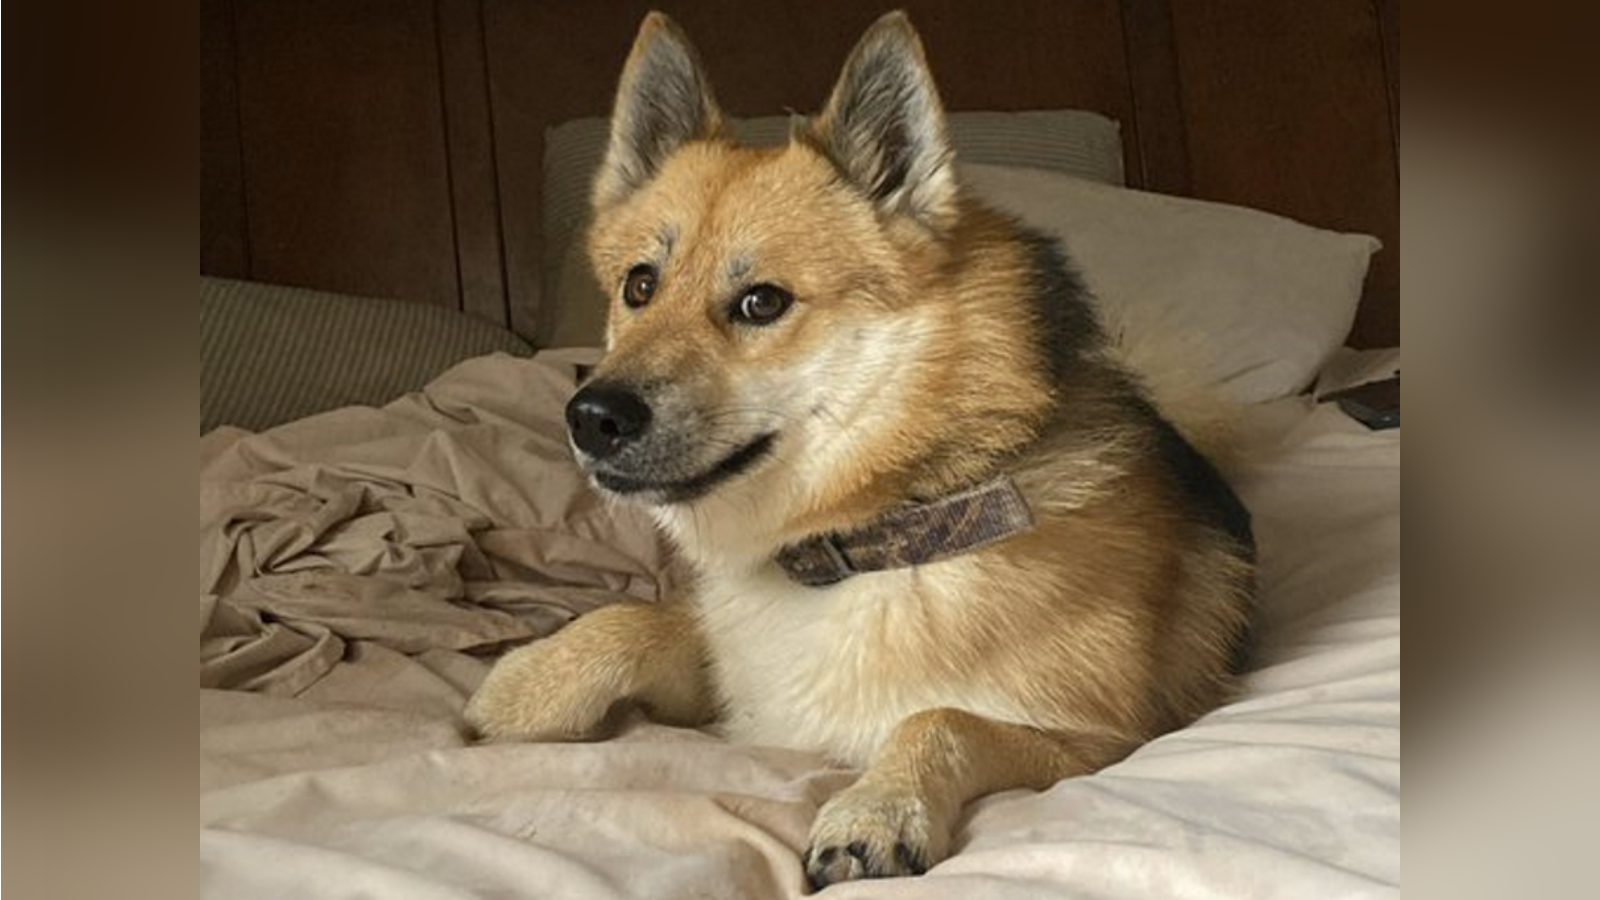
\includegraphics[width=\linewidth]{doge2.jpg}
\end{frame}
\end{document}
